\bodychapter{Applications}
\label{chp:app}

In this chapter we discuss two applications of elliptic curve cryptography,
    both of which benefit from the added security granted by the binary Edwards
    group law.
Moreover, they may be more attractive to implementors because they use binary
    Edwards curves rather than some other type; computers do work in binary,
    after all, so binary Edwards curves can lend themselves to efficient
    implementation in software or even hardware (e.g.
    \cite{chatterjee2011fpga}, \cite{kocabas2009hardware},
    \cite{kocabas2010implementation}).

\bodysection{Password Based Key Derivation}

\bodysubsection{Background}
Our first application is a password based key derivation function, or PBKDF.
Password safety is paramount in today's interconnected world; users log in to
    multiple workstations, websites, and services for communication, work,
    banking---the list goes on.
Despite its importance, password safety still a tricky technical subject, one
    that even experts get wrong sometimes; for example, according to
    \cite{arstechnica}, the IEEE exposed plaintext passwords in a public FTP
    directory ``for over a month.''
One way to securely store passwords is, somewhat paradoxically, to not store
    them at all.
Instead, a system can use a PBKDF to store different information derived from a
user's login credentials to authenticate them.

To quote \cite{percival2009stronger},
\begin{quote}
Password-based key derivation functions are used for two primary purposes:
    First, to hash passwords so that an attacker who gains access to a password
    file does not immediately possess the passwords contained therein; and
    second, to generate cryptographic keys to be used for encrypting and/or
    authenticating data.
\ldots Since all modern key derivation functions are constructed from hashes
    against which no non-trivial pre-image attacks are known, attacking the key
    derivation function directly is infeasible; consequently, the best attack
    in either case is to iterate through likely passwords and apply the key
    derivation function to each in turn.
Unfortunately, this form of ``brute force'' attack is quite liable to succeed.
Users often select passwords which have far less entropy than is typically
    required of cryptographic keys; a recent study found that even for web
    sites such as \texttt{paypal.com}, where---since accounts are often linked
    to credit cards and bank accounts---one would expect users to make an
    effort to use strong passwords, the average password has an estimated
    entropy of 42.02 bits, while only a very small fraction had more than 64
    bits of entropy.\footnote{The cited study is \cite{florencio2007large}.}
This is where a properly designed PBKDF comes in.
\end{quote}

As \cite{turan2010recommendation} says, ``the main idea of a PBKDF is to slow
    dictionary or brute force attacks on the passwords by increasing the time
    needed to test each password.''
Ideally, it should behave like a random mapping from passwords to possible
    data, which we'll called \textit{password hashes}, though this term is
    somewhat problematic.\footnote{Using ``hashes'' may lead one to think that
    using a general-purpose hash function like SHA-256 as a PBKDF is a good
    idea; as we'll see, this is not the case.}
To slightly borrow some of \cite{menezes1996handbook}'s exposition, ``a
    password, associated with each user (entity), is typically a string of 6 to
    10 or more characters the user is capable of committing to memory.''
In order to authenticate herself to the system in question, ``the user enters a
    (userid, password) pair'' to the system, which then uses this information
    in some way to compute the hash.
Once this computation is complete, the system checks the hash against the
    credentials it has stored for the supplied userid; if the hash matches the
    one on file, the user is granted access to the system.

Clearly a string of 6 to 10 memorable characters may not have enough entropy to
    qualify as cryptographically secure; therefore, a PBKDF should be designed
    to make the hash output look as random as possible.
Randomness alone isn't enough, however; as \cite{percival2009stronger} mentions
    above, cryptographic security can be compromised if the PBKDF is too
    computationally simple to perform; consider the following example.
\begin{ex}
Suppose an eavesdropper Eve manages to get her hands on the table of
\[
[\mathrm{userid}, \mathrm{hash}(\mathrm{password})]
\]
    pairs for Alice's system.
If Eve's desire to break into Alice's system isn't particularly time sensitive,
    she can simply grab a large file of likely passwords and hash them all
    until she finds a match in the second column of the table.
If Alice chose to use a general purpose message hashing algorithm for her
    PBKDF like SHA-3 (\cite{baum2012nist}), Eve may have the computational
    power to break into Alice's system soon enough to cause severe damage.
\end{ex}

One way to combat this ``dictionary attack'' is to widen the search space by
    \textit{salting} the hashes; for each userid, a system may instead store
    $\mathrm{hash}(\mathrm{password} \ast \mathrm{salt})$ for some operation
    $\ast$, typically string concatenation or bit exclusive-or, where the salt
    is a secret value known only to the system.
In this setup, a potential attacker would have to brute-force over all possible
    salts as well as all possible passwords, greatly increasing the work
    involved.
Even with salting, however, the speed of hash can still be an issue given
    today's technology.
There are a number of recent publications regarding cracking password hashes by
    brute force, many of which use the advanced parallel computing power
    granted by today's GPUs---see \cite{alnoonexecuting,
    gomez2010cryptanalysis, lim2004parallelization}, and
    \cite{zonenberg2009distributed}.

To make matters worse, the inevitable increase in computing power we experience
    as technology changes means that attackers will be able to attack any fixed
    PBKDF more and more easily as time goes by.
This means that a successful PBKDF should be tunable to meet this rising power
    available to would-be password crackers; as \cite{provos1999future} puts
    it, we are looking for a future-adaptable password scheme to ``keep up with
    hardware speeds.''
A secure PBKDF's computational cost ``must increase as hardware improves.''

One other successful PBKDF is \cite{provos1999future}'s \texttt{bcrypt}.
However, it isn't the final answer to the PBKDF problem; \texttt{bcrypt} is
    already under some scrutiny, and some alternatives have been proposed, the
    most notable of which is probably \cite{percival2009stronger}'s
    \texttt{scrypt}.
Like \texttt{scrypt}, our proposed PBKDF will incorporate a pseudorandom
    number generator.
It will also make use of binary Edwards curves; although they can be
    implemented rather efficiently, the inherent complexity of binary Edwards
    curves compared to the computer primitives of which typical hash functions
    are built adds to the security of our PBKDF.

\bodysubsection{Proposed PBKDF}
To further research into and development of secure PBKDFs, I propose we take a
    cue from NIST: look at a candidate scheme that is very different
    from what currently exists, so they won't (necessarily) be vulnerable to
    the same attacks, like NIST did with the recent SHA-3 competition.
Explaining some of the reasons for declaring \texttt{Keccak} the winner, they
    wrote
    \begin{quote}
    ``Keccak has the added advantage of not being vulnerable in the same ways
    SHA-2 might be,''says NIST computer security expert Tim Polk. ``An attack
    that could work on SHA-2 most likely would not work on Keccak because the
    two algorithms are designed so differently.'' \cite{baum2012nist}
    \end{quote}
In fact, we'll take even more from NIST's recent competition and present a
    variation on the Elliptic Curve Only Hash (ECOH, \cite{brown2008ecoh})
    which was submitted to the SHA-3 competition in 2008.
This variation makes some changes to the original algorithm to combat the
    main weakness that lost it the competition, viz. the second pre-image
    attack found in \cite{halcrow2009second, cryptoeprint:2009:168}.
At the same time, these changes ensure that while several different instances
    of our PBKDF can be parallelized, the algorithm itself is inherently serial
    and thus resists any further attempts at parallelization.

Specifically, the points $P_i$ and the values $X_1$ and $X_2$ presented in this
    section rely on the state of the algorithm at every step.
That is, each $P_i$ for $i > 0$ relies upon the previous $P_{i-1}$, and both
    $X_1$ and $X_2$ rely on the all of the $P_i$.
We also incorporate a pseudorandom number generator, not unlike other PBKDFs
    like \texttt{scrypt} \cite{percival2009stronger}.
As mentioned, these changes effectively ameliorate the second pre-image attack
    from \cite{cryptoeprint:2009:168}; they also have force the different
    stages of the hash to be computed serially, removing any chance of
    parallelization.
This makes our PBKDF more resilient in the face of processors that are no
    longer scaling up to greater speeds but out to more and more cores; for an
    offline attack, only multiple instances of our PBKDF can be run on a
    parallel machine or GPU.
The PBKDF itself can't be sped up.

Finally, we make some changes to the parameters involved.
Rather than sticking to an Elliptic curve in Weierstrass form, we make use of
    a binary Edwards curve; this makes the PBKDF more resistant to side-channel
    analysis.
We also remove the nondeterministic part of the \textit{Search} step of ECOH,
    instead using the ideas from \cite{icart2009hash} to deterministically map
    a field element to a point on our curve.
In doing so, we incorporate the birational map from \cite{moloneyefficient}.

Our PBKDF, called \texttt{ECOH's Echo}, takes in a salt $s$ and password $p$
    and makes use of the following parameters:
\begin{itemize}
\item   a pseudorandom number generator PRNG that can be seeded (primed with an
initial state)
\item   a block size $blen$, number of blocks/rounds $numblocks$, length $ilen$
    for integer bit representations, and an output length
\item   a finite field $\mathbb{F}_{2^n}$, an algebraic extension of
    $\mathbb{F}_2$ of degree $n$
\item   $a_2$ and $a_6$, two elements of $\mathbb{F}_{2^n}$ determining an
    elliptic curve in Weierstrass form
\item   $E$, the birationally equivalent binary Edwards curve
\item   $G$, a base point on $E$
\end{itemize}
Note that our parameters are not set in stone, but rather can be scaled up to
    larger sizes as potential attacking computing power increases.
We can increase our degree $n$ as well as the other parameters as the need
    arises.

We also make use of a number of maps:
\begin{itemize}
\item   $\pi$, a deterministic map from $K$ to $E$ (see \cite{icart2009hash}
    and \cite{moloneyefficient}) that takes a fixed number of steps
\item   A mapping $\omega: E \times \{X, Y\} \to K$, given by
\[
(Q, Z) \mapsto \frac{\left\lfloor Q + \left\lfloor \frac{Q.z}{2} \right\rfloor
    G \right\rfloor.z}{2} \bmod 2^{blen}
\]
    where $z = x$ if $Z = X$ and $y$ if $Z = Y$ (i.e., $Z$ picks out the
    coordinate).
This is an extension of the output mapping from the original ECOH submission
    (\cite{brown2008ecoh}) to work with either of a point's coordinates.
\item   A mapping $\varphi: E \to K$ given by $\varphi(Q) = \omega(Q, X)$ (not
    strictly needed, of course, this is just a specialization of $\omega$)
\item   A mapping $\psi: E \to \mathbb{F}_2$ given by $\psi(Q) = \omega(Q, Y)
    \& 1$, the least significant bit of $\omega(Q, Y)$
\end{itemize}
Before we move on, let's flesh out the details of the map $\pi$.
Take \cite{icart2009hash}'s $f_{a_2, a_6}:\mathbb{F}_{2^n} \to
    W(\mathbb{F}_{2^n})$ where $W$ is an elliptic curve in the Weierstrass form
\[
v^2 + uv = u^3 + a_2u^2 + a_6
\]
    defined by $z \mapsto (u, v)$ such that
\begin{align*}
\alpha  &=  a_2 + z + z^2\\
u       &=  (\alpha^4 + \alpha^3 + a_6)^{\sfrac{1}{3}} + \alpha\\
v       &=  zu + \alpha^2
\end{align*}
    and combine it with \cite{moloneyefficient}'s birational equivalence to
    create $\pi$ via $z \mapsto (u, v) \mapsto (x, y)$.\footnote{We use this
    one instead of the original given in \cite{bernstein2008binary} due to its
    having only one exceptional point ($\infty$ which won't show up here) and
    being more efficient in implementation.} 
This gives us a direct mapping $\pi: \mathbb{F}_{2^n} \to E(\mathbb{F}_{2^n})$
    that inherits all of the cryptographically desirable properties of
    $f_{a_2, a_6}$ since the birational equivalence has no exceptional points
    save $\infty$.
Moreover, it's more secure than the \textit{Search} step of ECOH, since this
    was a nondeterministic map that would take an indeterminate amount of
    steps.
As always, we strive to minimize the leakage of extra information through
    side-channels.

We'll first give a more na\"ive version of \texttt{ECOH's Echo}.

\bodysubsubsection{Na\"ive Version}
Execution proceeds as follows: first, our PRNG is seeded with the exclusive-or
    (XOR) of the password and salt.\footnote{Strictly speaking, there is an
    encoding involved in making an integer value out of the password. In our
    reference implementation below, we make the usual choice of treating the
    password as a string of ASCII-encoded bytes and build an integer out of
    that.}
Each block $O_i$ is generated in the following way: given an integer $i$,
    append the $ilen$-bit representation of $i$ to a $blen - ilen$ long stream
    of pseudorandom bits from PRNG.
Second, we initialize a point $P_0$ from the initial block $O_0$ by setting it
    to be $\pi(O_0)$.
We then iterate for $numblocks - 1$ rounds, setting $P_i$ to be $\pi(O_i \oplus
    i \oplus \varphi(P_{i-1}))$.
Next we update $numblocks$, saving
\[
numblocks \oplus \left(\sum\nolimits_0^{numblocks - 1}2^i\psi(P_i)\right)
\]
    in its place.
After that, $X_1$ and $X_2$ are defined to be $\pi(numblocks)$ and
\[
\pi\left(numblocks \oplus
    \left[\bigoplus\nolimits_0^{numblocks-1} O_i\right]
\right)
\]
    respectively.
Finally, we define $Q$ to be the sum
\[
X_1 + X_2 + \sum\nolimits_0^{numblocks-1}P_i
\]
    and output $\varphi(Q)$.

\bodysubsubsection{Memory Efficient Version}
Though it's simpler to follow, the above version of our PBKDF is not as
    efficient with regards to memory as it could be.
We needn't store all the intermediate points $P_i$, for instance, if we instead
    introduce two temporary variables $Y_1$ and $Y_2$ that will be used to
    build $X_1$ and $X_2$ later.
After seeding PRNG as before, let $(O, Y_1, Y_2) = (O_0, numblocks, numblocks)$
    and set $Q = P = \pi(O)$.
Then we iterate for $i \in \{1, \ldots, numblocks - 1\}$, setting
\begin{align*}
O   &=  O_i\\
P   &=  \pi(O \oplus i \oplus \varphi(P))\\
Y_1 &=  Y_1 + 2^i\psi(P)\\
Y_2 &=  Y_2 \oplus O\\
Q   &=  Q + P
\end{align*}
    at each step of the loop.
Finally, let $X_1 = \pi(Y_1)$, $X_2 = \pi(Y_1 \oplus Y_2)$, and $Q = Q + X_1 +
    X_2$.
As before, we output $\varphi(Q)$.

\bodysubsection{Algorithm Pseudocode and Diagrams}
We give a description of \texttt{ECOH's Echo} in algorithms (\ref{alg:naive})
    and (\ref{alg:good}).
Diagrams of the flow of the rounds in the more efficient description are given
    in Figures (\ref{fig:first_round}) and (\ref{fig:other_rounds}).

\begin{Algorithm}
\caption{ECOH's Echo, Na\"ive version}
\label{alg:naive}
\begin{algorithmic}
    \Function{ECOH's Echo}{$p, s$}
        \State PRNG.salt$(s \oplus p)$
        \State $P_0 \gets \pi(O_0)$
        \For{$i \gets 1 \texttt{ to } numblocks - 1$}
            \State $P_i \gets \pi\left(O_i \oplus i \oplus
                \varphi(P_{i-1})\right)$
        \EndFor
        \State $numblocks \gets numblocks \oplus \left(\sum_0^{numblocks - 1}
            2^i\psi(P_i)\right)$
        \State $X_1 \gets \pi(numblocks)$
        \State $X_2 \gets \pi\left(numblocks \oplus
            \left[\bigoplus_0^{numblocks-1} O_i\right]\right)$
        \State $Q \gets X_1 + X_2 + \sum_0^{numblocks-1}P_i$
        \State \Return $\varphi(Q)$
    \EndFunction
\end{algorithmic}
\end{Algorithm}

\begin{Algorithm}
\caption{ECOH's Echo, Memory-Efficient Version}
\label{alg:good}
\begin{algorithmic}
    \Function{ECOH's Echo}{$p, s$}
        \State PRNG.salt$(s \oplus p)$
        \State $O \gets O_0$
        \State $Y_1 \gets numblocks$
        \State $Y_2 \gets numblocks$
        \State $P \gets \pi(O)$
        \State $Q \gets P$
        \For{$i \gets 1 \texttt{ to } numblocks - 1$}
            \State $O \gets O_i$
            \State $P \gets \pi\left(O \oplus i \oplus \varphi(P)\right)$
            \State $Y_1 \gets Y_1 \oplus 2^i\psi(P)$
            \State $Y_2 \gets Y_2 \oplus O$
            \State $Q \gets Q + P$
        \EndFor
        \State $X_1 \gets \pi(Y_1)$
        \State $X_2 \gets \pi\left(Y_1 \oplus Y_2\right)$
        \State $Q \gets Q + X_1 + X_2$
        \State \Return $\varphi(Q)$
    \EndFunction
\end{algorithmic}
\end{Algorithm}

\begin{figure}[htbp]
    \centering
    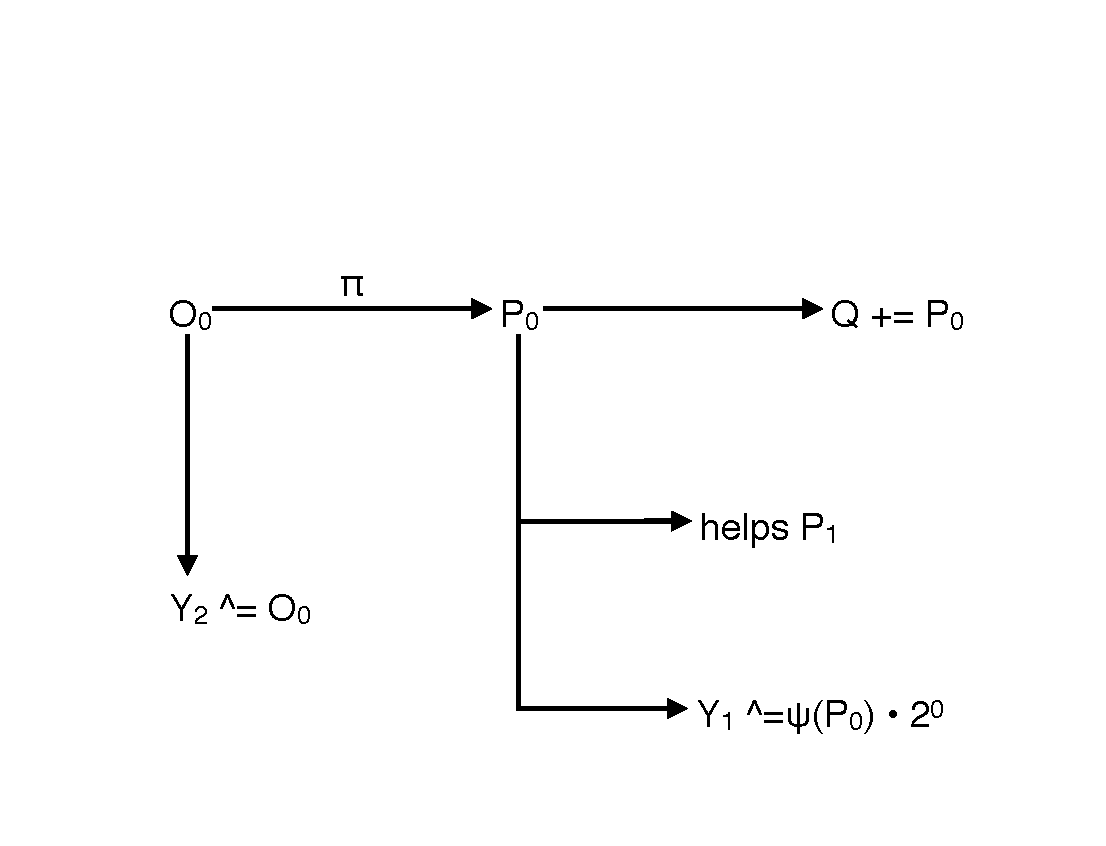
\includegraphics[scale=0.5]{figures/ecoh_echo.pdf}
    \caption{First round of \texttt{ECOH's Echo}}
    \label{fig:first_round}
\end{figure}

\begin{figure}[htbp]
    \centering
    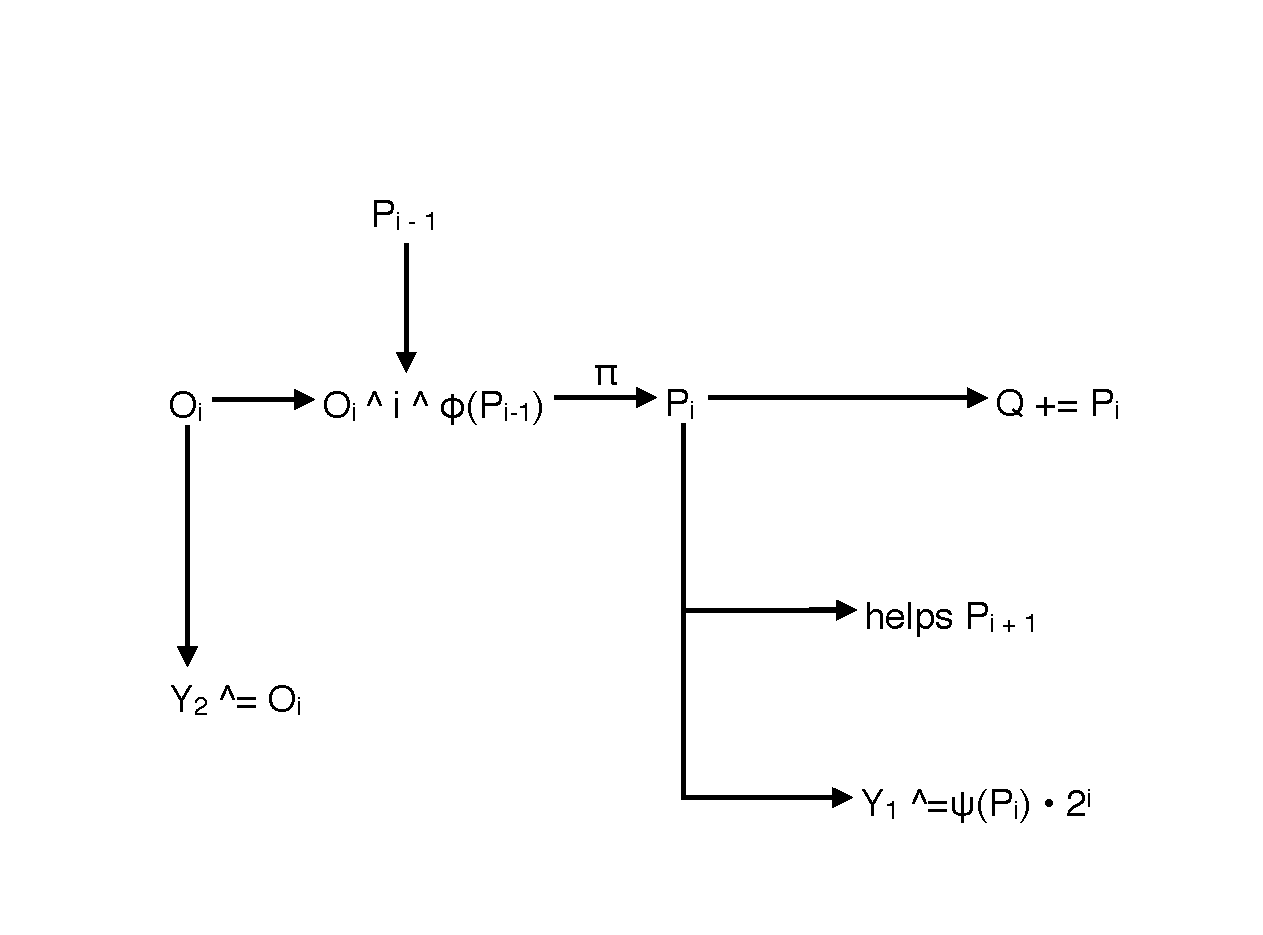
\includegraphics[scale=0.5]{figures/ecoh_echo2.pdf}
    \caption{Subsequent rounds of \texttt{ECOH's Echo}}
    \label{fig:other_rounds}
\end{figure}

\newpage
\bodysubsection{\texttt{ECOH's Echo} Reference Implementation}
Finally, we provide a reference implementation of \texttt{ECOH's Echo} using
    our software library \texttt{e2c2}.
For more on \texttt{e2c2}, see Appendix \ref{chp:src}.
\lstinputlisting[caption={ECOH's Echo}]{backmatter/src/ecoh_echo.cc}

\bodysection{Compartmented ID-Based Secret Sharing and Signcryption}

Another application of elliptic curves and elliptic curve cryptography is using
    pairings for identity-based schemes, like those first suggested in
    \cite{boneh2001identity}.\footnote{A previous of this section has been
    posted to the International Association for Cryptologic Research's
    cryptology eprint archive (\texttt{http://eprint.iacr.org/2012/528}) and
    has been submitted for consideration to the Information Processing Letters
    Journal for consideration for publication.}
In \cite{li2006id}, Li, Xin, and Hu describe an ID-based signcryption scheme
    that uses a bilinear map to accomplish $(t, n)$ shared unsigncryption with
    the help of Shamir's secret sharing scheme.
Here we describe a way to extend Li et. al.'s construction into a
    \textit{compartmented scheme}.
For our compartmented scheme, suppose the organization $\mathcal{O}$ is split
    into several compartments $\mathcal{C}_i$, $i \in \{1, \ldots, t\}$.
In order to unsigncrypt a message sent to $\mathcal{O}$, at least one member of
    each of the $t$ compartments must participate; without the cooperation of
    at least one member from each compartment, the message cannot be
    unsigncrypted.
What's more, each member $\mathcal{M}_{ij} \in \mathcal{C}_i$ gets
    different information; therefore, although any $\mathcal{M}_{ij}$ can
    participate equally, the compartment $\mathcal{C}_i$ is in fact split up
    so that all of its potential participants have something unique to
    contribute.

In what follows, we will make the following changes to the terminology and
    notation of \cite{li2006id}: uppercase letters will denote points on an
    elliptic curve $E$ over a predetermined finite field $K$, lowercase letters
    will denote elements in the multiplicative group $\mu_n$ of $n$th roots of
    unity, Greek letters are used for elements of $\mathbb{F}_q$, and script
    letters generally denote compartments or members thereof.
Moreover, $\widehat{e}$ is a pairing function from $E \times E \to \mu_n =
    \mathbb{F}_{q^k}^\ast/\mathbb{F}_{q^k}^{\ast n}$.

\bodysubsection{Preliminaries}
Here we briefly discuss the basic tools needed for our scheme, namely
\begin{enumerate}
\item Bilinear Diffie-Hellman Problems
\item Identity-based encryption
\item Shamir's threshold scheme
\item Signcryption
\item Baek \& Zheng's zero knowledge proof for the equality of two discrete
    logarithms based on a bilinear map
\end{enumerate}
We also cite relevant references for readers who would like more in-depth
    coverage of these interesting topics.

\bodysubsubsection{Bilinear Diffie-Hellman Problems}
As \cite{menezes1996handbook} writes, bilinear maps were first used in
    cryptography to weaken systems rather than create them.
In \cite{menezes1993reducing}, the authors showed that ``the discrete logarithm
    problem for an elliptic curve over a finite field $\mathbb{F}_q$ can be
    reduced to the discrete logarithm problem in some extension field
    $\mathbb{F}_q^k$.''
For a particular class of curves called \textit{supersingular} curves, this was
    a particularly devastating attack.
Fortunately for elliptic curve cryptography, not all curves are supersingular.

The basic idea behind this attack was that if $Q = \ell P$, then
\[
\widehat{e}(P, Q)
    = \widehat{e}(P, P)^\ell 
\]
    so we can solve the resulting discrete logarithm problem (or Diffie-Hellman
    problem) in a different group instead, one where logarithms might be
    computed more easily.
As such, we need to pick our groups $E$ and $\mu_n$ such that the Decisional
    Diffie-Hellman Problem is difficult in $\mu_n$ and the following problems
    are difficult in $(E, \mu_n, \widehat{e})$:
\begin{prob}[Computational Diffie-Hellman Problem]
Suppose $P$ is a generator of a large subgroup of $E$ and $\alpha \in
    \mu_n = \widehat{e}(P, P)$.
Given $Q, R \in E$ such that $Q = bP$ and $R = cP$, compute $bc$ via $\beta =
    \alpha^b = \widehat{e}(P, Q)$ and $\gamma = \alpha^c = \widehat{e}(P, R)$.
\end{prob}
\begin{prob}[Decisional Diffie-Hellman Problem]
Suppose $P$ is a generator of a large subgroup of $E$ and $\alpha \in \mu_n =
    \widehat{e}(P, P)$.
Given $Q, R, S \in E$ such that $Q = bP$ and $R = cP$, determine which of the
    following is true  via $\beta = \alpha^b = \widehat{e}(P, Q)$ and $\gamma =
    \alpha^c = \widehat{e}(P, R)$:
\begin{enumerate}
\item   $S = bcP$ (so $\delta = \widehat{e}(P, S)$ is equal to $\alpha^{bc}$)
\item   $S = dP$ for some $d$ chosen uniformly at random from $\mathbb{Z}_n$
    independently of $b$ and $c$.
\end{enumerate}
\end{prob}
These problems are currently believed to be difficult if the size $n$ of our
    groups is chosen large enough.

\bodysubsubsection{Identity-Based Encryption}
In \cite{shamir1985identity}, Shamir proposed an interesting problem: he
    ``asked for a public key encryption scheme in which the public key can be
    an arbitrary string.'' \cite{boneh2001identity}
Shamir wished to simplify the management of digital certificates in e-mail and
    other systems; as the authors of \cite{boneh2001identity} write, he wished
    to have a system such that ``when Alice sends mail to Bob at
    \texttt{bob@hotmail.com} she simply encrypts her message using the public
    key string `\texttt{bob@hotmail.com}','' thereby removing the need for
    interacting with any sort of management or external cryptographic
    infrastructure on a per-message basis.
One of the most satisfying solutions to date comes from Boneh and Franklin.
The Weil pairing was used in Boneh and Franklin's scheme in
    \cite{boneh2001identity}; readers are referred to this paper for more.

In \cite{shamir1985identity} and \cite{boneh2001identity}, the protocols and
    schemes consist of four stages: \textit{Setup}, \textit{Extract},
    \textit{Encrypt}, and \textit{Decrypt}.
We follow the notation of \cite{li2006id} in the description of our scheme,
    though, with the four stages \textit{Setup}, \textit{Extraction},
    \textit{Signcryption}, and \textit{Unsigncryption}.
Before we get to the protocol, however, there is more background to cover.

\bodysubsubsection{Shamir's Threshold Scheme}

In \cite{shamir1979share}, Shamir developed a simple and elegant method to
    share a secret piece of information amongst $n$ people such that no less
    than some threshold value $t$ of them must cooperate to recover that
    secret.
This scheme uses polynomial interpolation over a finite field; if we suppose
    that the secret piece of information $s$ is encoded as some element of the
    field, we then construct a random polynomial $f$ of degree $t - 1$ such
    that $f(0) = s$ (so $s$ is the constant term).
If we give the pair $(i, f(i))$ to the $i$th person in our scheme, for $1 \le i
    \le n$, then via Lagrange interpolation any group of $t$ people can first
    reconstruct the polynomial $f$ and then evaluate $f(0)$ to recover $s$.
Furthermore, because no group of $t - 1$ or less people will suffice to recover
    the polynomial, this scheme is information-theoretically secure.
For more, see the original paper \cite{shamir1979share};
    \cite{simmons1990really} extends the idea of secret sharing to multipartite
    and compartmented schemes, while \cite{brickell1990some, ghodosi1998secret,
    iftene2005compartmented} and \cite{iftene2007general} discuss some ways to
    share secrets in various settings.
To our knowledge, however, none of these include identity-based encryption and
    the next topic: signcryption.

\bodysubsubsection{Signcryption}

In \cite{zheng1997digital}, the author put forth a new idea that combines the
    steps of digitally signing and encrypting a message---traditionally two
    separate procedures---that drastically reduces the computational and
    communication costs involved.
Later work extended this idea to include other cryptographically desirable
    features such as non-repudiation, public-verifiability, and forward
    security (see \cite{li2006id}).
Recently made into an international standard, signcryption has gained
    increasing popularity with researchers and implementers alike.
For more information, see the original \cite{zheng1997digital};
    \cite{zheng1998construct} demonstrates how to implement signcryption using
    rational points on elliptic curves over finite fields.
Even more information, including an extensive bibliography, can be found online
    at \texttt{signcryption.org}.

\bodysubsubsection{Baek \& Zheng's zero knowledge proof}

In this section, $\mathcal{O}$ stands for the neutral element on an Edwards
    curve $E$ instead of the organization in question.
Per \cite{baek2004identity} and \cite{li2006id}, the zero knowledge proof of
    membership for the language
\[
L_{\mathtt{EDLog}_{P, \widetilde{P}}^{E}}
    \stackrel{\mathrm{def}}{=}
    \{(x, \widetilde{x}) \in \mu_n \times \mu_n \mid \log_g x = \log_{
        \widetilde{g}}\widetilde{x} \}
\]
    (where $g = \widehat{e}(P, P)$ and $\widetilde{g} = \widehat{e}\left(
    \widetilde{P}, \widetilde{P}\right)$ for generators $P$ and $\widetilde{P}$
    of a large additive cyclic subgroup $E(K)$ of order $\#E = n$) ensure the
    robustness of our threshold decryption.
Provided that the Decisional Diffie-Hellman problem is hard in $\mu_n$ and the
Computational and Decisional Bilinear Diffie-Hellman Problems are difficult in
    $(E, \mu_n, \widehat{e})$, the basic idea is as follows: suppose both the
    Prover and the Verifier receive the tuple $\left(P, \widetilde{P}, g,
    \widetilde{g}\right)$ and the pair $(k, \widetilde{k}) \in
    L_{\mathtt{EDLog}_{P, \widetilde{P}}^{\mu_n}}$.
Moreover, suppose the Prover knows a secret $S \in E\setminus\{\mathcal{O}\}$
    such that $k = \widehat{e}(S, P)$ and $\widetilde{k} = \widehat{e}(S,
    \widetilde{P})$; then
\begin{enumerate}
\item The Prover chooses at random an element $R \in E\setminus\{\mathcal{O}\}$
    computes $a = \widehat{e}(R, P)$ and $\widetilde{a} = \widehat{e}(R,
    \widetilde{P})$, and sends $a$ and $\widetilde{a}$ to the Verifier.
\item The verifier picks $\gamma \in \mathbb{F}_q^\ast$ at random and sends it
    to the Prover.
\item The Prover computes $T = R + \gamma S$ and sends it to the Verifier.
    If (and only if) the two equalities
\[
ak^\gamma = \widehat{e}(T, P)
\qquad
\widetilde{a}\widetilde{k}^{\gamma} = \widehat{e}(T, \widetilde{P})
\]
    hold, the Verifier believes that the Prover knows the secret $S$ since
\[
\widehat{e}(T, P)
    = \widehat{e}(R + \gamma S, P)
    = \widehat{e}(R, P)\widehat{e}(S, P)^\gamma
    = ak^\gamma
\]
    and
\[
\widehat{e}(T, \widetilde{P})
    = \widehat{e}(R + \gamma S, \widetilde{P})
    = \widehat{e}(R, \widetilde{P})\widehat{e}(S, \widetilde{P})^\gamma
    = \widetilde{a}\widetilde{k}^\gamma
\]
\end{enumerate}

For more, including how to adapt the above into a non-interactive zero
    knowledge proof, see \cite{baek2004identity}.


\bodysubsection{The Proposed Compartmented Scheme}

Suppose we have an organization $\mathcal{O}$ consisting of $n$ people split
    into $t$ compartments $\mathcal{C}_i$, each consisting of members
    $\mathcal{M}_{ij}$.
In addition, we have a Private Key Generator ($\mathcal{P}$) who acts as the
    trusted authority and a sender Alice ($\mathcal{A}$) who wishes to send a
    message to the compartments $\mathcal{C}_i \subset \mathcal{O}$.
There are four stages: \textit{Setup}, \textit{Extraction},
    \textit{Signcryption}, and \textit{Unsigncryption}.


\bodysubsubsection{Setup}

$\mathcal{P}$ first chooses our two groups of large prime order $n$: $E$ and
    $\mu_n$.
$\mathcal{P}$ also picks a generator $P$ of $E$ and a number of  hash
    functions:\footnote{$H_1$ can be the one from \cite{icart2009hash}}
\begin{align*}
    H_1 &: \{0, 1\}^\ast \to E\\
    H_2 &: \mu_n \to \{0, 1\}^\ast\\
    H_3 &: \{0, 1\}^\ast \times \mu_n \to \mathbb{F}_q^\ast\\
\end{align*}
Finally, $\mathcal{P}$ chooses a secret master key $s \in \mathbb{F}_q^\ast$,
    computes $P_{pub} = sP$, and publishes the tuple
\[
(E, \mu_n, n, \widehat{e}, P, P_{pub}, H_1, H_2, H_3, E, D)
\]
    where $E$ and $D$ are the encryption and decryption steps of some fast
    symmetric key cipher (like AES; see \cite{daemen2002design}).


\bodysubsubsection{Extraction}

In what follows, given an ID (identifying information considered as a bit
    string), the public key $\mathcal{P}$ generates for that ID is $Q_{ID} =
    H_1(ID)$, the private signcryption key is $S_{ID} = s^{-1}Q_{ID}$, and the
    private decryption key is $D_{ID} = sQ_{ID}$.

Since $\mathcal{P}$ uses $ID_{\mathcal{O}}$ to compute $Q_{\mathcal{O}}$,
    $S_{\mathcal{O}}$, and $D_{\mathcal{O}}$ and wishes to pass information to
    each $\mathcal{C}_i$ in such a way that some cooperation is required to put
    $D_{\mathcal{O}}$ back together, she randomly picks $R_k \in E \setminus\{
    \mathcal{O}\}$, $k \in \{1, \ldots, t - 1\}$, and constructs a function $f:
    \{0, 1\}^\ast \to E$ via $f(u) = D_{\mathcal{O}} + \sum_1^{t-1} u^k R_k$
    (treating $u$ as the binary representation of some positive integer).
Then, for each $\mathcal{C}_i \subset \mathcal{O}$, $\mathcal{P}$:
\begin{enumerate}
\item Computes $D_i = f(ID_i)$, the private decryption key for $\mathcal{C}_i$
\item Computes $y_i = \widehat{e}(D_i, P)$, the public verification key for
    $\mathcal{C}_i$
\item For each $\mathcal{M}_{ij} \in \mathcal{C}_i$, $\mathcal{P}$:
    \begin{enumerate}
    \item Chooses a random $\mu_{ij} \in \mathbb{F}_q^\ast$
    \item Privately sends $\mathcal{M}_{ij}$ the triple
    \begin{math}
    (D_i, P_{ij}, y_{ij}) = \left(D_i, (1 + \mu_{ij})D_i, y_i^{\mu_{ij}}\right)
    \end{math}
    \end{enumerate}
\item Finally, $\mathcal{P}$ publishes the table
\begin{align*}
\{(ID_i, y_i, \{(ID_{ij}, y_{ij})\}\}
    =\; &(ID_1, y_1, (ID_{1, 1}, y_{1, 1}), (ID_{1, 2}, y_{1, 2}), \ldots\\
        &(ID_2, y_2,  (ID_{2, 1}, y_{2, 1}), (ID_{2, 2}, y_{2, 2}), \ldots\\
        &\vdots
\end{align*}
\end{enumerate}


\bodysubsubsection{Signcryption}

To send the message $m$ to $\mathcal{O}$, Alice computes the signcrypted text
    $(c, r, S)$ as follows:
\begin{enumerate}
\item She chooses a random $x \in \mathbb{F}_q^\ast$
\item $k_1 = \widehat{e}(P, Q_\mathcal{A})^x$
\item $k_2 = H_2(\widehat{e}(Q_\mathcal{A}, Q_{\mathcal{O}})^x)$
\item $c = E_{k_2}(m)$
\item $r = H_3(c, k_1)$
\item $S = (x - r)S_\mathcal{A}$
\end{enumerate}


\bodysubsubsection{Unsigncryption}

After at least one member $\mathcal{M}_{ij}$ from each of the $t$ compartments
    $\mathcal{C}_i$ assemble, they first verify Alice's signature; then each
    $\mathcal{M}_{ij}$ individually

\begin{enumerate}
\item Computes $k_1^\prime = \widehat{e}(S, P_{pub})\widehat{e}(Q_\mathcal{A},
    P)^r$
\item Accepts Alice's signature if and only if $r = H_3(c, k_1^\prime)$
\end{enumerate}

Next, each $\mathcal{M}_{ij}$ picks two random points $B_{ij}, T_{ij} \in
    E$ and uses $B_{ij}$ to certify that they belong to $\mathcal{C}_i$ and
    $T_{ij}$ to certify their decryption share.
While the latter is accomplished in exactly the same manner as in
    \cite{li2006id}, $\mathcal{M}_{ij}$ does the former as follows:
\begin{enumerate}
\item[3.] Construct credentials $\kappa_{ij}$ using $B_{ij}$, where
\[
\kappa_{ij}
    = (\widetilde{P}_{ij}, z_{ij})
    = \left(P_{ij} + B_{ij}, y_{ij}\widehat{e}(B_{ij}, P)\right)
\]
\item[4.] Send credentials $\kappa_{ij}$ to each of the other
    $\mathcal{M}_{k\ell}$
\item[5.] Check each of $\mathcal{M}_{k\ell}$'s credentials by testing whether
\[
y_k = \frac{\widehat{e}(\widetilde{P}_{k\ell}, P)}{z_{k\ell}}
\]
\end{enumerate}

Once everyone's credentials are established, the rest of unsigncryption
    continues as in \cite{li2006id}.


\bodysubsection{Analysis of Scheme}

We discuss the effects to correctness, security, and efficiency of the changes
    we have made to \cite{li2006id}'s original scheme.
As such, our analysis is based on that of \cite{li2006id}, especially where it
    makes use of \cite{baek2004identity}'s zero knowledge proof of membership.


\bodysubsubsection{Correctness}

Observe that
\begin{align*}
\frac{\widehat{e}(\widetilde{P}_{ij}, P)}{z_{ij}}
    &=  \frac{\widehat{e}(P_{ij}, P)\widehat{E}(B_{ij}, P)}
            {y_{ij}\widehat{e}(B_{ij}, P)}\\
    &=  \frac{\widehat{e}\left((1 + \mu_{ij})D_k, P\right)}
            {y_k^{\mu_{ij}}}\\
    &=  \frac{\widehat{e}(D_k, P)\widehat{e}(D_k, P)^{\mu_{ij}}}
            {y_k^{\mu_{ij}}}\\
    &=  \widehat{e}(D_k, P)\\
    &=  y_k
\end{align*}

So $\kappa_{ij}$ does indeed certify that $\mathcal{M}_{ij}$ belongs to and can
    speak for the compartment $\mathcal{C}_k$.
The correctness of the rest of our scheme can be proven in exactly the same
    manner as \cite{li2006id}.


\bodysubsubsection{Security}

Because the signcryption process in our scheme is the same as in
    \cite{li2006id} (which in turn is the same as in \cite{chow2004efficient}),
    our scheme has the same existential unforgeability against chosen plaintext
    attacks in the random oracle model as those schemes, provided that the
    Computational Bilinear Diffie-Hellman Problem is difficult in the groups
    and pairing underlying the implementation of our scheme.

What's more, our scheme doesn't change the level of confidentiality either;
    assuming the Decisional Bilinear Diffie-Hellman Problem is hard in $(E,
    \mu_n, \widehat{e})$, our scheme enjoys the same indistinguishability
    against adaptive chosen ciphertext attacks in the random oracle model.
During unsigncryption, no less than $t$ cooperating members of different
    compartments suffice to recover the key $k_2$ (and hence the message).
Giving different randomly obfuscated versions of the same information to
    members of the same compartment does nothing to lessen this fact.
Recovery of $D_\mathcal{O}$ is also computationally infeasible due to the
    difficulty of inverting the pairing $\widehat{e}$.
Finally, the use of Baek and Zheng's zero knowledge proof ensures that each
    member participating in unsigncryption is protected against the possibility
    of dishonesty from any of the others.

The public verifiability of our extended scheme remains intact, since any third
    party can verify the signature via the first two steps of the
    \textit{Unsigncryption} stage.

We also still keep forward security, since it remains difficult to compute
    $k_2^\prime$ without $D_\mathcal{O}$, even if $S_\mathcal{A}$ is leaked.


\bodysubsubsection{Efficiency}
With a slight modification to \cite{li2006id}'s notation, let $T_p$, $T_m$, and
    $T_e$ be the computing time required for calculating a pairing, point
    multiplication, and exponentiation, respectively.
Note that our scheme still requires $2T_p + T_m + 2T_e$ for signcryption and
    $(2t + 4)T_p + T_m + (3t - 1)T_e$ for $\mathcal{M}_{ij}$, just like the
    original scheme.
The main bottleneck in this scheme is the random point choices performed by
    $\mathcal{P}$; if we assume that $\mathcal{P}$ has a fast pseudorandom
    number generator, then the time this takes is essentially $(2n + 1)T_m$,
    just like in \cite{li2006id}.

The efficiency picture can be improved, though; instead of having $\mathcal{P}$
    choose each $\mathcal{M}_{ij}$'s point, it could instead choose $t$ points
    and send them to $t$ secondary generators $P_i$, one for each compartment.
These secondary generators can then randomize those points and distribute the
    relevant information to the members of their respective compartments.
Though this doesn't reduce the work involved (and it requires having more
    trusted authorities, or rather semi-trusted authorities), it does allow
    our scheme to parallelize one of its major, one-time steps.
Hence our scheme lends itself better to implementation using modern computing
    methods (i.e. parallel computation) than does \cite{li2006id}.

\bodysubsection{Conclusion}

In this section we demonstrated how a small modification to Li, Xin, and Hu's
    scheme (\cite{li2006id}) extends it into a compartmented scheme, allowing a
    sender to address a message to an organization $\mathcal{O}$ and requiring
    different compartments $\mathcal{C}_i \subset \mathcal{O}$ to cooperate for
    the message's recovery.
In doing so, we do not lose any of the security or efficiency features of
    \cite{li2006id}'s scheme---in fact, we can even parallelize one of the main
    stages.
To our knowledge, this scheme is the first that combines identity-based
    encryption, Shamir's secret sharing, and signcryption into a compartmented
    sharing scheme that can be implemented with available algorithms and
    software.

This scheme incorporates a naturally parallelizable step, and is likewise
    naturally applicable to modern situations.
For instance, this scheme could very easily be used in cloud computing to
    synchronize information passed to different groups or clusters from a
    single host.
As another example, one could use this scheme for authenticated and signcrypted
    communication in a business setting; the shared secret could be an expected
    return message to acknowledge receipt of an important document or the
    scheduling of an important meeting.
There is still room for future work.
We hope to investigate deeper into questions such as increasing the efficiency
    of our scheme or reducing the reliance upon the trusted private key
    generator $\mathcal{P}$.
